\lesson{4}{Apr 12 2022 Tue (16:27:32)}{Part 1: Intro to Trig Functions}
\label{lec_4:part_1_intro_to_trig_functions}

\begin{definition}[Unit Circle]
  \label{def:unit_circle}

  A \textbf{unit circle} is a circle with a radius of $1$ unit.

  \begin{figure}[H]
    \centering

    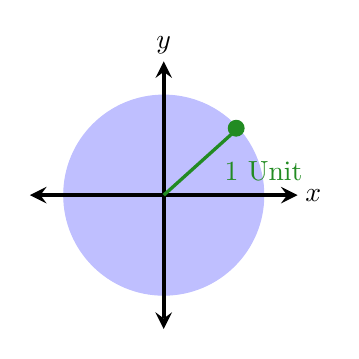
\begin{tikzpicture}
      \draw[draw=blue!25!white,fill=blue!25!white] (0,0) circle (0.5in);

      \draw (0,1.9) node[anchor=center] {$y$};
      \draw (1.9,0) node[anchor=center] {$x$};

      \draw[stealth-stealth,ultra thick] (0,1.7) -- (0,-1.7);
      \draw[stealth-stealth,ultra thick] (1.7,0) -- (-1.7,0);
      \draw[very thick,ForestGreen] (0,0) -- (1,0.9);
      \draw [ForestGreen,fill=ForestGreen,radius=0.1] (0.92,0.85) circle;

      \draw (0.65,0.3) node[ForestGreen,anchor=west] {$1$ Unit};
    \end{tikzpicture}

    \caption{Unit Circle}
    \label{fig:unit_circle}
  \end{figure}
\end{definition}

Now we can define the $\sin$ and $\cos$ functions.

\begin{note}
  There are $4$ other trigonometric functions that can be defined in terms of
  $\sin$ and $\cos$ functions so first we'll get familiar with $\sin$ and $\cos$
  and then later in the next lecture \ref{les_5:part_2_intro_to_trig_functions}
  we'll define the $4$ other trigonometric functions.
\end{note}

\begin{definition}[Sine and Cosine]
  \label{def:sine_and_cosine}

  The \textbf{sine function}, denoted $\sin(\theta)$, associates each angle
  $\theta$ with the vertical coordinate of the point $P$ specified by $\theta$
  on the circumference of a unit circle.

  The \textbf{cosine function}, denoted $\cos(\theta)$, associates each angle
  $\theta$ with the horizontal coordinate of the point $P$ specified by
  $\theta$ on the circumference of a unit circle.

  So the point $P$ in the figure below has coordinates:
  \[ (x, y) = (\cos(\theta), \sin(\theta)) \].

  \begin{figure}[H]
    \centering

    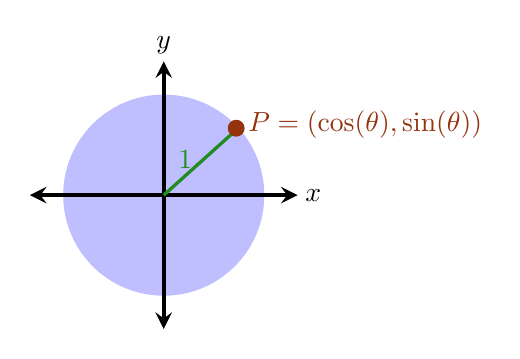
\begin{tikzpicture}
      \draw[draw=blue!25!white,fill=blue!25!white] (0,0) circle (0.5in);

      \draw (0,1.9) node[anchor=center] {$y$};
      \draw (1.9,0) node[anchor=center] {$x$};

      \draw[stealth-stealth,ultra thick] (0,1.7) -- (0,-1.7);
      \draw[stealth-stealth,ultra thick] (1.7,0) -- (-1.7,0);

      \draw[very thick,ForestGreen] (0,0) to node[left] {$1$} (1,0.9);
      \draw[RawSienna,fill=RawSienna,radius=0.1] (0.92,0.85) circle;
      \draw (0.95,0.9) node[RawSienna,anchor=west] {$P = (\cos(\theta), \sin(\theta))$};
    \end{tikzpicture}

    \caption{Sin and Cos on Graph}
    \label{fig:sin_and_cos}
  \end{figure}
\end{definition}

\begin{exc}[Solution \ref{sol:angle_of_theta}]
  \label{exc:angle_of_theta}

  The angle of $\theta$ specifies the point
  $P = \left(-\frac{3}{5}, \frac{4}{5}\right)$ on the circumference
  of a unit circle. Find $\sin(\theta)$ and $\cos(\theta)$.
\end{exc}

Let's determine the signs of the sin and cos functions in the four
quadrants:

\begin{itemize}
  \label{item:signs_in_the_4_quadrants}

  \item When the terminal side of angle $\theta$ is in Quadrant I, both the $x$
    and $y$ coordinates of point $P$ are positive. Therefore, \textbf{if
    $\theta$ is in Quadrant I, $\cos(\theta) > 0$ and $\sin(\theta) > 0$}

  \item When the terminal side of angle $\theta$ is in Quadrant II, the $y$
    coordinate of point $P$ is positive but the $x$ coordinate is negative.
    Therefore, \textbf{if $\theta$ is in Quadrant II, $\cos(\theta) < 0$ and
    $\sin(\theta) > 0$}

  \item When the terminal side of angle $\theta$ is in Quadrant III, both the
    $x$ and $y$ coordinates of point $P$ are negative. Therefore, \textbf{if
    $\theta$ is in Quadrant IIII, $\cos(\theta) < 0$ and $\sin(\theta) < 0$}

  \item When the terminal side of angle $\theta$ is in Quadrant IIII, the $x$
    coordinate of point $P$ is positive but the $y$ coordinate is negative.
    Therefore, \textbf{if $\theta$ is in Quadrant IIII, $\cos(\theta) > 0$ and
    $\sin(\theta) < 0$}
\end{itemize}

\begin{figure}[htpb]
  \centering

  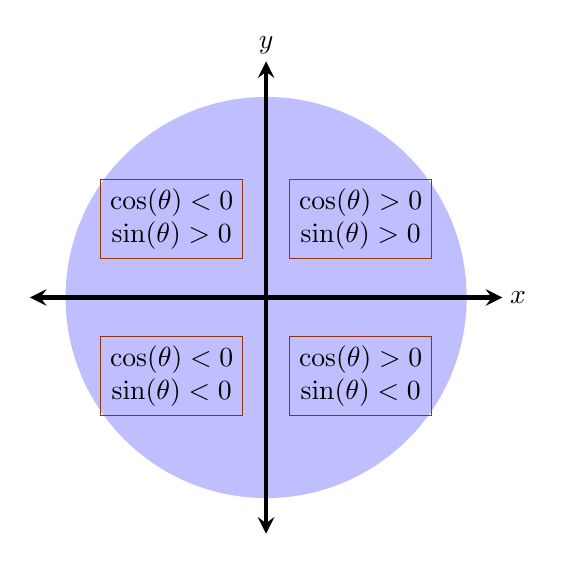
\begin{tikzpicture}[every text node part/.style={align=center}]
    \draw[draw=blue!25!white,fill=blue!25!white] (0,0) circle (1in);

    \draw (0,3.2) node[fill=white,anchor=center] {$y$};
    \draw (3.2,0) node[fill=white,anchor=center] {$x$};

    \draw[stealth-stealth,ultra thick] (0,3) -- (0,-3);
    \draw[stealth-stealth,ultra thick] (3,0) -- (-3,0);

    \draw (1.2,1) node[rectangle,draw=RawSienna]
      {$\cos(\theta) > 0$ \\ $\sin(\theta) > 0$};
    \draw (-1.2,1) node[rectangle,draw=RawSienna]
      {$\cos(\theta) < 0$ \\ $\sin(\theta) > 0$};
    \draw (-1.2,-1) node[rectangle,draw=RawSienna]
      {$\cos(\theta) < 0$ \\ $\sin(\theta) < 0$};
    \draw (1.2,-1) node[rectangle,draw=RawSienna]
      {$\cos(\theta) > 0$ \\ $\sin(\theta) < 0$};
  \end{tikzpicture}

  \caption{Quadrants of a Graph}
  \label{fig:quadrants}
\end{figure}

Now let's find the sin and cos of a few particular angles. The easiest points
for us to find on the unit circle are points where the circumference of the
circle intersects the coordinate axes. Let's start by finding the corresponding
sin and cos values.

\begin{note}
  \label{nte:sin_and_cos}

  Keep in mind that {\color{red}cos} represents the {\color{red}x-coordinate}
  and {\color{green}sin} represents the {\color{green}y-coordinate}.
\end{note}

\begin{itemize}
  \label{item:find_sin_and_cos}

  \item The angle $\theta = 90^{\circ}$ ($\theta = \frac{\pi}{2}$ radians),
    specifies the point $(0, 1)$ on the circumference of a unit circle. Thus
    \ldots

    \[ \cos \left(\frac{\pi}{2}\right) = 0 \qquad \sin \left(\frac{\pi}{2}\right) = 1 \].

    \begin{figure}[H]
      \centering

      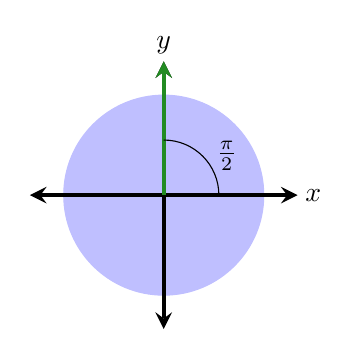
\begin{tikzpicture}
        \draw[draw=blue!25!white,fill=blue!25!white] (0,0) circle (0.5in);

        \draw (0,1.9) node[fill=white,anchor=center] {$y$};
        \draw (1.9,0) node[fill=white,anchor=center] {$x$};

        \draw[stealth-stealth,ultra thick] (0,1.7) -- (0,-1.7);
        \draw[stealth-stealth,ultra thick] (1.7,0) -- (-1.7,0);
        \draw[-stealth,ultra thick,ForestGreen] (0,0) -- (0,1.7);

        \draw (0.7,0) arc[start angle=0,end angle=90,radius=0.7];
        \node at (0.8,0.5) {$\frac{\pi}{2}$};
      \end{tikzpicture}

      \caption{}
      \label{fig:90_degree}
    \end{figure}

  \item The angle $\theta = 180^{\circ}$ ($\theta = \pi$ radians), specifies the
    point $(-1, 0)$ on circumference of a unit circle. Thus \ldots

    \[ \cos (\pi) = -1 \qquad \sin (\pi) = 0 \].

    \begin{figure}[H]
      \centering

      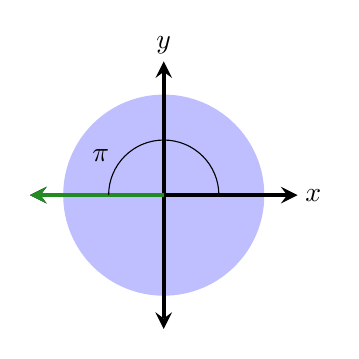
\begin{tikzpicture}
        \draw[draw=blue!25!white,fill=blue!25!white] (0,0) circle (0.5in);

        \draw (0,1.9) node[fill=white,anchor=center] {$y$};
        \draw (1.9,0) node[fill=white,anchor=center] {$x$};

        \draw[stealth-stealth,ultra thick] (0,1.7) -- (0,-1.7);
        \draw[stealth-stealth,ultra thick] (1.7,0) -- (-1.7,0);
        \draw[-stealth,ultra thick,ForestGreen] (0,0) -- (-1.7,0);

        \draw (0.7,0) arc[start angle=0,end angle=180,radius=0.7];
        \node at (-0.8,0.5) {$\pi$};
      \end{tikzpicture}

      \caption{}
      \label{fig:180_degree}
    \end{figure}

  \item The angle $\theta = 270^{\circ}$ ($\theta = \frac{3\pi}{2}$ radians),
    specifies the point $(0, -1)$ on the circumference of a unit circle. Thus
    \ldots

    \[ \cos \left(\frac{3\pi}{2}\right) = 0 \qquad \sin \left(\frac{3\pi}{2}\right) = -1 \].

    \begin{figure}[H]
      \centering

      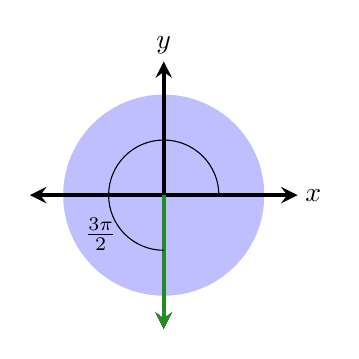
\begin{tikzpicture}
        \draw[draw=blue!25!white,fill=blue!25!white] (0,0) circle (0.5in);

        \draw (0,1.9) node[fill=white,anchor=center] {$y$};
        \draw (1.9,0) node[fill=white,anchor=center] {$x$};

        \draw[stealth-stealth,ultra thick] (0,1.7) -- (0,-1.7);
        \draw[stealth-stealth,ultra thick] (1.7,0) -- (-1.7,0);
        \draw[-stealth,ultra thick,ForestGreen] (0,0) -- (0,-1.7);

        \draw (0.7,0) arc[start angle=0,end angle=270,radius=0.7];
        \node at (-0.8,-0.5) {$\frac{3\pi}{2}$};
      \end{tikzpicture}

      \caption{}
      \label{fig:270_degree}
    \end{figure}

  \item The angle $\theta = 360^{\circ}$ ($\theta = 2\pi$ radians), specifies
    the point $(1, 0)$ on the circumference of a unit circle. Thus \ldots

    \[ \cos (2\pi) = 1 \qquad \sin (2\pi) = 0 \].

    \begin{figure}[H]
      \centering

      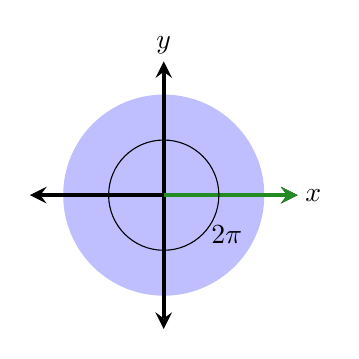
\begin{tikzpicture}
        \draw[draw=blue!25!white,fill=blue!25!white] (0,0) circle (0.5in);

        \draw (0,1.9) node[fill=white,anchor=center] {$y$};
        \draw (1.9,0) node[fill=white,anchor=center] {$x$};

        \draw[stealth-stealth,ultra thick] (0,1.7) -- (0,-1.7);
        \draw[stealth-stealth,ultra thick] (1.7,0) -- (-1.7,0);
        \draw[-stealth,ultra thick,ForestGreen] (0,0) -- (1.7,0);

        \draw (0.7,0) arc[start angle=0,end angle=360,radius=0.7];
        \node at (0.8,-0.5) {$2\pi$};
      \end{tikzpicture}

      \caption{}
      \label{fig:360_degree}
    \end{figure}
\end{itemize}

Notice that angles of measure $2\pi$ radians and $0$ radians specify the same
point: $(1, 0)$. Thus, the sin and cos values for $2\pi$ and $0$ radians are the
same:

\[ \cos (2\pi) = \cos (0) = 1 \qquad \textrm{and} \qquad \sin (2\pi) = \sin (0) = 0\].

Since any angle $\theta$ and $\theta + 2\pi$ specify the same point on the unit
circle, the sin and cos values of $\theta$ and $\theta + 2\pi$ are the same.
Therefore, the period of the sin and cos function is $2\pi$ radians.

\begin{theorem}
  For all $\theta$, $\sin (\theta) = \sin (\theta + 2\pi)$ and $\cos (\theta) =
  \cos(\theta + 2\pi)$ so the period of both $s (\theta) = \sin (\theta)$ and
  $c (\theta) = \cos (\theta)$ is $2\pi$ radians.
\end{theorem}

Now, we'll sketch graphs of the sin and cos functions.

\newpage

We first start by organizing the function values in a table:

\begin{table}[htpb]
  \label{tab:values_of_sin_and_cos}
  \centering

  \begin{tabular}{|c|c|c|c|c|c|c|c|c|c|}
    \hline
    $\theta$ (degrees) & $0^{\circ}$ & $90^{\circ}$ & $180^{\circ}$ & $270^{\circ}$ & $360^{\circ}$ & $450^{\circ}$ & $540^{\circ}$ & $630^{\circ}$ & $720^{\circ}$ \\
    \hline
    $\theta$ (radians) & $0$ & $\frac{\pi}{2}$ & $\pi$ & $\frac{3\pi}{2}$ & $2\pi$ & $\frac{5\pi}{2}$ & $3\pi$ & $\frac{7\pi}{2}$ & $4\pi$ \\
    \hline
    $y = \cos (\theta)$ & $1$ & $0$ & $-1$ & $0$ & $1$ & $0$ & $-1$ & $0$ & $1$ \\
    \hline
    $y = \sin (\theta)$ & $0$ & $1$ & $0$ & $-1$ & $0$ & $1$ & $0$ & $-1$ & $0$ \\
    \hline
  \end{tabular}

  \caption{Values of Sin and Cos}
\end{table}

Here's how it looks like when we graph:

\begin{figure}[htpb]
	\centering

	\begin{tikzpicture}
		\begin{axis}[
				my axis style,
				width=\textwidth,
				height=.5\textwidth,
			]
			\addplot[
				domain=-10:10,
        blue,
				thick,
				<->
			]
			{sin(deg(x))};

			\addplot[
				domain=-10:10,
        red,
				thick,
				<->
			]
			{cos(deg(x))};
		\end{axis}
	\end{tikzpicture}

  \caption{The graph of {\color{red}$y = \cos(\theta)$} and {\color{blue}$y = \sin(\theta)$}}
  \label{fig:the_graph_of_y_cos_theta_and_y_sin_theta_2}
\end{figure}

Notice that the graphs of $y = \cos (\theta)$ and $y = \sin (\theta)$ are very
similar. In fact, if we shift $y = \sin (\theta)$ to the left $\frac{\pi}{2}$
units, we'll obtain the graph of $y = \cos (\theta)$. This means that:

\[ \cos = \sin \left(\theta + \frac{\pi}{2}\right) \].

Similarly, if we shift $y = \cos (\theta)$ to the right $\frac{\pi}{2}$ units,
we'll obtain the graph of $y = \sin (\theta)$. This means that:

\[ \sin = \cos \left(\theta - \frac{\pi}{2}\right) \].

\begin{definition}[Identity]
  \label{def:identity}

  An \textbf{identity} is an equation that is true for all values in the domains
  of the involved expressions.
\end{definition}

\begin{tcolorbox}
  \begin{center}
    Some important trig identities
  \end{center}

  \begin{minipage}[t]{.50\textwidth}
      \begin{itemize}
      \item $\cos (\theta) = \cos (\theta + 2\pi)$
      \item $\sin (\theta) = \cos \left(\theta - \frac{\pi}{2}\right)$ 
      \item $\cos (-\theta) = \cos (\theta)$
      \item $\cos (\theta) = \cos (2\pi - \theta)$
    \end{itemize}
  \end{minipage}%
  \begin{minipage}[t]{.50\textwidth}
   \begin{itemize}
      \item $\sin (\theta) = \sin (\theta + 2\pi)$
      \item $\cos (\theta) = \sin \left(\theta + \frac{\pi}{2}\right)$ 
      \item $\sin (-\theta) = -\sin (\theta)$
      \item $\sin (\theta) = \cos (\pi - \theta)$
    \end{itemize}
  \end{minipage}
\end{tcolorbox}

We can generalize the definitions of sin and cos functions so that they are
applicable to circles of any size, rather than only for unit circles.

\begin{definition}[More Applicable version of Sin and Cos]
  \label{def:more_applicable_version_of_sin_and_cos}
  If the point $T = (x, y)$ is specified by the angle $\theta$ on the
  circumference of a circle of radius $r$ then:

  \[ \cos (\theta) = \frac{x}{r} \qquad \textrm{and} \qquad \sin (\theta) = \frac{y}{r} \].

  \begin{note}
    \label{nte:more_applicable_version_of_sin_and_cos}

    If $r = 1$, then this definition $\cos (\theta)$ and $\sin (\theta)$ are
    equivalent to what we saw at the beginning of this lecture.

    \[ \cos (\theta) = \frac{x}{r} = \frac{x}{1} = x \qquad \textrm{and} \qquad \sin (\theta) = \frac{y}{r} = \frac{y}{1} = y \].
  \end{note}

  If we solve the equations $\cos (\theta) = \frac{x}{r}$ and $\sin (\theta) =
  \frac{y}{r}$ for $x$ and $y$, we can obtain the coordinates of a point on the
  circumference of a circle of any $r$ :

  \[ \cos (\theta) = \frac{x}{r} \implies x = r \cos (\theta) \qquad \textrm{and} \qquad \sin (\theta) = \frac{y}{r} \implies y = r \sin (\theta) \].

  If the point $T = (x, y)$ is specified by the angle $\theta$ on the
  circumference of a circle of radius, $r$, then:

  \[ x = r \cos (\theta) \qquad \textrm{and} \qquad y = r \sin(\theta) \].
\end{definition}

\begin{exc}[Solution \ref{sol:using_r_cos_and_r_sin}]
  \label{exc:using_r_cos_and_r_sin}

  A circle with a radius of $6$ units is given. The point $Q$ is specified by
  the angle $\alpha$. Use the sin and cos function to express the exact
  coordinates of point $Q$.

  \begin{figure}[H]
    \centering

    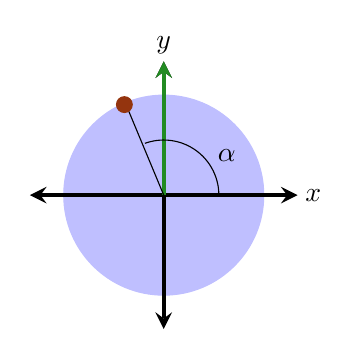
\begin{tikzpicture}
      \draw[draw=blue!25!white,fill=blue!25!white] (0,0) circle (0.5in);

      \draw (0,1.9) node[fill=white,anchor=center] {$y$};
      \draw (1.9,0) node[fill=white,anchor=center] {$x$};

      \draw[stealth-stealth,ultra thick] (0,1.7) -- (0,-1.7);
      \draw[stealth-stealth,ultra thick] (1.7,0) -- (-1.7,0);
      \draw[-stealth,ultra thick,ForestGreen] (0,0) -- (0,1.7);

      \draw (0.7,0) arc[start angle=0,end angle=110,radius=0.7];
      \node at (0.8,0.5) {$\alpha$};
      \draw (0,0) -- (-0.5,1.2);

      \draw[fill=RawSienna,RawSienna] (-0.5,1.15) circle (0.1);
    \end{tikzpicture}

    \caption{}
    \label{fig:circle_with_radius_of_6_units}
  \end{figure}
\end{exc}

\vspace*{0.1in}

Recall that the cos and sin functions represent the horizontal and vertical
coordinates of a point on the circumference of a unit circle. This situation
creates a right triangle with hypotenuse of length $1$ unit and side-lengths of
$\cos (\theta)$ and $\sin (\theta)$ units.

\begin{figure}[htpb]
  \centering

  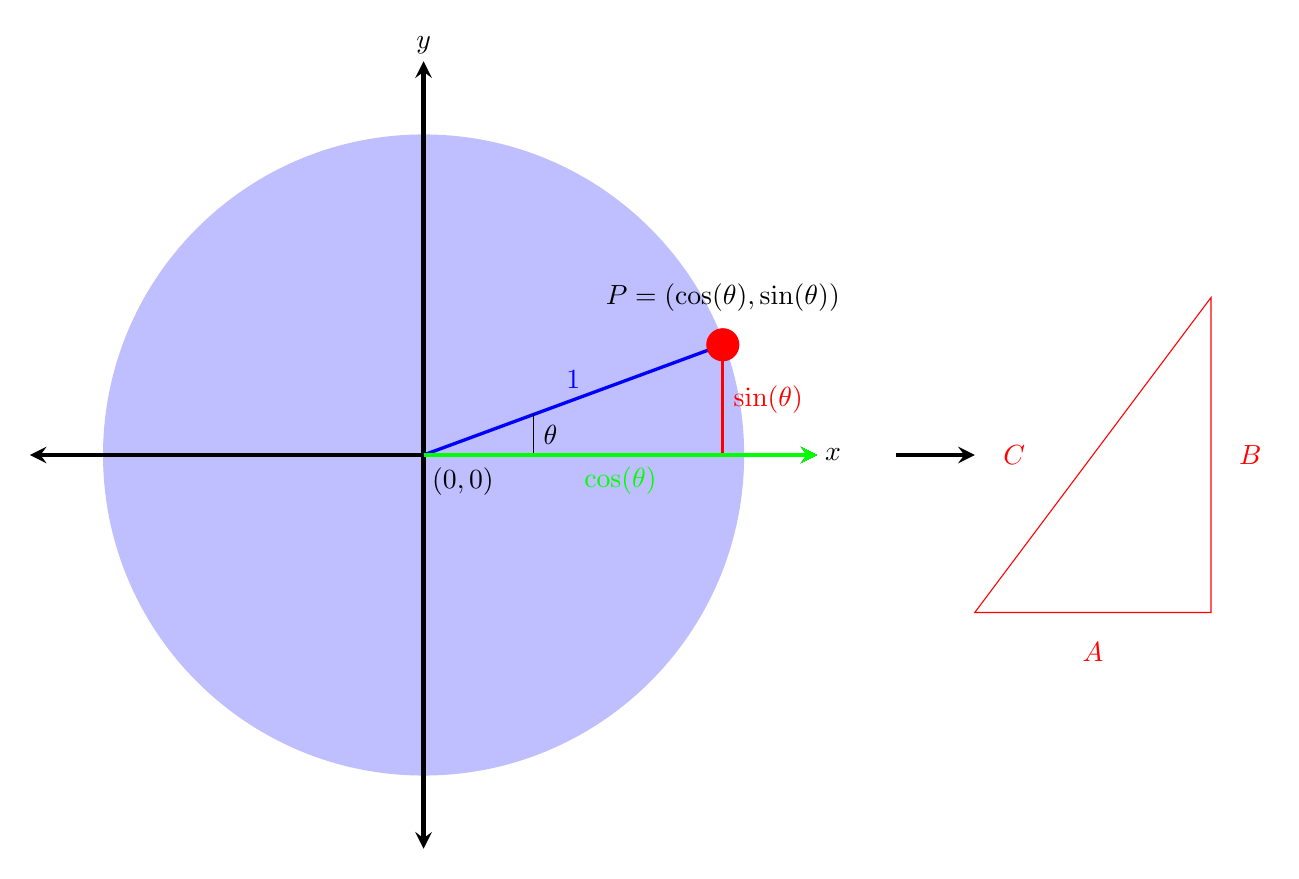
\begin{tikzpicture}
    \draw[draw=blue!25!white,fill=blue!25!white] (0,0) circle (1.60in);
    \draw (0.50,-0.04) node[fill=blue!25!white,anchor=north] {$(0,0)$};
    \draw (0,5.2) node[fill=white,anchor=center] {$y$};
    \draw (5.2,0) node[fill=white,anchor=center] {$x$};
    \draw[stealth-stealth,ultra thick] (0,5) -- (0,-5);
    \draw[stealth-stealth,ultra thick] (5,0) -- (-5,0);
    \draw[blue,very thick] (0,0) to node[anchor=south] {$1$} (3.8,1.4);
    \draw[draw=red,fill=red] (3.8,1.4) circle (0.08in);
    \draw (3.8,2) node[anchor=center] {$P = (\cos (\theta), \sin (\theta))$};
    \draw[very thick,red] (3.8,1.4) to node[anchor=west] {$\sin (\theta)$} (3.8,0);
    \draw (1.4,0.52) to node[right] {$\theta$} (1.4,0);
    \draw[ultra thick,green,-stealth] (0,0) to node[anchor=north] {$\cos (\theta)$} (5,0);
    \draw[-stealth,ultra thick] (6,0) -- (7,0);
    \draw[red] (10,-2) coordinate[label=] (c)
          -- (10,2) coordinate[label=] (b)
          -- (7,-2) coordinate[label=] (a)
          -- cycle;
    \draw[red] (8.5,-2.5) node[anchor=center] {$A$};
    \draw[red] (10.5,0) node[anchor=center] {$B$};
    \draw[red] (7.5,0) node[anchor=center] {$C$};
  \end{tikzpicture}

  \caption{Diagram of a Circle}
  \label{fig:diagram_of_a_circle}
\end{figure}

Now we can apply the Pythagorean Theorem to this right triangle. First let's
review the Pythagorean Theorem:

\begin{theorem}[Pythagorean Theorem]
  \label{thrm:pythagorean_theorem}

  If the sides of a right triangle are labeled. Then \ldots

  \begin{figure}[H]
    \centering

    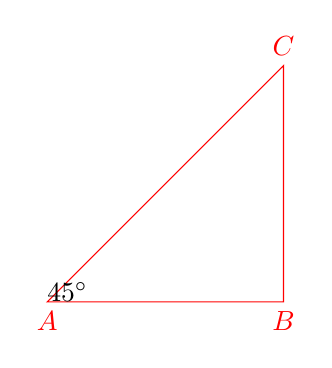
\begin{tikzpicture}
      \draw[red]  (0,0) coordinate[label=below:$A$] (a) --
                  (3,0) coordinate[label=below:$B$] (c) --
                  (3,3) coordinate[label=above:$C$] (b) -- cycle;
      % \pic[my angle, "$\alpha=\SI{45}{\degree}$"] {angle = c--a--b};
      \tkzMarkAngle[mark=none](c,a,b);
      \tkzLabelAngle[pos=0.6](c,a,b){$45^{\circ}$};
    \end{tikzpicture}

    \caption{Right Triangle}
    \label{fig:pythagorean_theorem}
  \end{figure}

  \[ a^{2} + b^{2} = c^{2} \].
\end{theorem}

Applying the Pythagorean Theorem to the right triangle we obtain what is called
the Pythagorean Identity:
\[ \sin^{2}(\theta) + \cos^{2}(\theta) = 1 \].
When we use exponents in trigonometric functions we can use unusual notation.
Instead of using parentheses around the entire expression, we can put the
exponents between the letters that name the function and the input for the
function. Thus, we can write an expression like $(\sin (\theta))^{2}$ as
$\sin^{2} (\theta)$. We can use this notation to express the Pythagorean
Identity:

\begin{notation}
  \[ \theta \in \mathbb{R} \textrm{, } \sin^{2} (\theta) + \cos^{2} (\theta) = 1 \].
\end{notation}

\begin{exc}[Solution \ref{sol:find_cos}]
  \label{exc:find_cos}

  If $\sin (A) = \frac{1}{3}$ and $\frac{\pi}{2} < A < \pi$, which means $A$ is
  in Quadrant II, find $\cos (A)$.
\end{exc}

\newpage
